% !TEX root = ../../book.tex

\chapter{Multivariate Time Series Models}

The methods developed in this chapter are natural extensions of the methods presented in Chapter 2 in the multivariate setting. But the underlying data is of large dimension and hence they present some unique challenges. These include unwieldy estimation problems as well as making meaningful interpretation of the estimates. But these methods are essential to address portfolio construction and trading issues. We want to present some basic tools in multivariate regression and tools for dimension-reduction, which provide a foundation for modeling multiple time series. Although multivariate ARMA models are well-studied in the literature, the focus has been on the multivariate (vector) autoregressive (VAR) models which falls neatly in the framework of multivariate regression with constraints on the regression coefficient matrices that account for stationarity. Thus a good understanding of multivariate regression will lay a solid foundation for studying VAR models.


In the area of multivariate analysis, there are two broad themes that have emerged over time. one that typically involves exploring the variations in a set of interrelated variables and two, involves investigating the simultaneous relationships between two or more sets of variables. In either case, the themes involve explicit modeling of the relationships or dimension-reduction of the sets of variables. The multivariate regression introduced in Section 3.1 and its variants are the preferred tools for the parametric modeling and descriptive tools such as principal components or canonical correlations are the tools used for addressing dimension-reduction issues (Section 3.2). Both act as complementary tools and data analyst may want to make use of these tools for a thorough analysis of multivariate data. 


\section{Multivariate Regression} 


We begin with the general multivariate linear model,
	\begin{equation}\label{eqn:5lmyk}
	Y_t = C X_t + \epsilon_t
	\end{equation}
where $Y_t=(Y_{1t},\ldots,Y_{mk})'$ is an $m \times 1$ vector of responsive variables and $X_k=(X_{1t},\ldots,X_{nt})'$ is an $n \times 1$ vector of predictors, $C$ is an $m \times n$ coefficient matrix and $\epsilon_t=(\epsilon_{it}, \ldots, \epsilon_{mt})'$ is the $m \times 1$ vector of random errors. We assume $E(\epsilon_t)=0$ and $\Cov(\epsilon_t)=\Sigma_{\epsilon \epsilon}$ is a $m \times m$ positive definite covariance matrix. The errors are independent over `$t$', the time index. Thus if we arrange the data and error as matrices,
	\begin{equation}\label{eqn:5yyt}
	Y=[Y_1,\ldots,Y_T], X=[X_1,\ldots,X_T] \text{ and }\epsilon=[\epsilon_1, \ldots,\epsilon_T]
	\end{equation}
and if $e=\text{vec}(\epsilon')$,
	\begin{equation}\label{eqn:5Ee0}
	E(e)=0, \Cov(e)= \Sigma_{\epsilon \epsilon} \otimes I_T
	\end{equation}
where the symbol $\otimes$ signifies the Kronecker's product. 


The unknown parameters in model (\ref{eqn:5lmyk}) are the elements of the regression coefficient matrix $C$ and the error covariance matrix $\Sigma_{\epsilon \epsilon}$. These can be estimated by the method of least squares, or equivalently, the method of maximum likelihood under the assumption of normality of the $\epsilon_k$. Note we can rewrite the model (\ref{eqn:5lmyk}) in terms of the complete data matrices $\mathbf{Y}$ and $\mathbf{X}$ as
	\begin{equation}\label{eqn:rewrite}
	\mathbf{Y} = C \mathbf{X} + \mathbf{\epsilon}
	\end{equation}
The least squares estimates are obtained by minimizing
	\begin{equation}\label{eqn:minimize}
	e'e=\text{tr}(\epsilon\epsilon')=\text{tr}[(\mathbf{Y}-C\mathbf{X})(\mathbf{Y}-C\mathbf{X})']=\text{tr}\left[\sum_{t=1}^T \epsilon_t \epsilon_t'\right]
	\end{equation}
where $\text{tr}(A)$ denotes the trace of a square matrix $A$, that is, the sum of the diagonal elements of $A$. This yields a unique solution for $C$ as
	\begin{equation}\label{eqn:solution}
	\tilde{C}=\mathbf{Y} \mathbf{X}' (\mathbf{X}\mathbf{X}')^{-1} = \left(\dfrac{1}{T} \mathbf{Y}\mathbf{X}'\right) \left(\dfrac{1}{T} \mathbf{X}\mathbf{X}' \right)^{-1}
	\end{equation}
Hence, it can be seen from the form of (\ref{eqn:solution}) the rows of the matrix $C$ are estimated by the least squares regression of each response variable on the predictor variables and therefore the covariances among the response variables do not enter into the estimation. The multivariate regression is essentially a series of multiple regressions. 


For maximum likelihood (ML) estimation, the criterion that must be minimized to estimate $C$ is 
	\begin{equation}\label{eqn:mintrace}
	\text{tr}\left(\Sigma^{-1}_{\epsilon\epsilon'}\right)=\text{tr}\left[ \Sigma_{\epsilon\epsilon}^{-1/2} (\mathbf{Y}-C\mathbf{X})(\mathbf{Y}-C\mathbf{X})' \Sigma_{\epsilon\epsilon}^{-1/2}\right]
	\end{equation}
which yields the same solution for $C$ as given in (\ref{eqn:solution}). The ML estimator of the error covariance matrix $\Sigma_{\epsilon\epsilon}$ is obtained from the least squares residuals $\hat{\mathbf{\epsilon}}=\mathbf{Y}- \tilde{C} \mathbf{X}$ as $\tilde{\Sigma}_{\epsilon\epsilon}= \frac{1}{T}(\mathbf{Y}-\tilde{C}\mathbf{X})(\mathbf{Y}-\tilde{C}\mathbf{X})' \equiv \frac{1}{T}S$, where $S= \sum_{t=1}^T \hat{\epsilon}_t \hat{\epsilon}_t'$ is the error sum of squares matrix, and $\hat{\epsilon}_t= Y_t - \tilde{C} \mathbf{X}_t$, $t=1,\ldots,T$, are the least squares residual vectors. An unbiased estimator of $\Sigma_{\epsilon\epsilon}$ is obtained as 
	\begin{equation}\label{eqn:5unbiased}
	\overline{\Sigma}_{\epsilon\epsilon} = \dfrac{1}{T-n} \,\hat{\epsilon} \hat{\epsilon}' = \dfrac{1}{T-n} \sum_{t=1}^T \hat{\epsilon}_t \hat{\epsilon}_t'.
	\end{equation}


\noindent\textbf{Inference Properties:} \\


Under the assumption that the matrix of predictor variables $\mathbf{X}$ is fixed and nonstochastic, properties of the least squares estimator $\tilde{C}$ in (\ref{eqn:solution}) can readily be derived. If $X_t$ is a stochastic vector, the LS estimator $\tilde{C}$ can be viewed as conditional on fixed observed values of the $X_t$. First, $\tilde{C}$ is an unbiased estimator of $C$, $E(\tilde{C})=C$ and $\Cov(\tilde{C}_{(i)}, \tilde{C}_{(j)})=\sigma_{ij}(\mathbf{X}\mathbf{X}')^{-1}$ for $i,j=1,\ldots,m$, where $\sigma_{ij}$ denotes the $(i,j)$th element of the covariance matrix $\Sigma_{\epsilon\epsilon}$, since $\Cov(\mathbf{Y}_{(i)}, \mathbf{Y}_{(i)})=\sigma_{ij} I_T$. The distributional properties of $\tilde{C}$ follow easily from multivariate normality of the error terms $\epsilon_t$. Specifically, we consider the distribution of $\text{vec}(\tilde{C}')$, where the ``vec'' operation transforms an $m \times n$ matrix into an $mn$-dimensional column vector by stacking the columns of the matrix below each other. 


\begin{result}\label{res:1}
For the model (\ref{eqn:5lmyk}) under the normality assumption on the $\epsilon_k$, the least squares estimator $\tilde{C}=\mathbf{Y} \mathbf{X}'(\mathbf{X} \mathbf{X}')^{-1}$ is the same as the maximum likelihood estimator of $C$, and the distribution of the least squares estimator $\tilde{C}$ is such that 
	\begin{equation}\label{eqn:distlsq}
	\text{vec}(\tilde{C}') \sim N(\text{vec}(C'), \Sigma_{\epsilon\epsilon} \otimes (\mathbf{X} \mathbf{X}')^{-1}).
	\end{equation}
Note, in particular, that this result implies that the $j$th row of $\tilde{C}$, $\tilde{C}_{(j)}'$, which is the vector of least squares estimates of regression coefficients for the $j$th response variable, has the distribution $\tilde{C}_{(j)} \sim N(C_{(j)}, \sigma_{jj}(\mathbf{X}\mathbf{X}')^{-1})$. The inference on the elements of the matrix $C$ can be made using the result in (\ref{eqn:distlsq}). In practice, because $\Sigma_{\epsilon\epsilon}$ is unknown, a reasonable estimator such as the unbiased estimator in (\ref{eqn:5unbiased}) is substituted for the covariance matrix in (\ref{eqn:distlsq}).


We shall also indicate the likelihood ratio procedure for testing simple linear hypotheses regarding the regression coefficient matrix. Consider $\mathbf{X}$ partitioned as $\mathbf{X}=[\mathbf{X}_!', \mathbf{X}_2']$ and corresponding $C=[C_1,C_2]$, so that the model (\ref{eqn:rewrite}) is written as $\mathbf{Y}=C_1 \mathbf{X}_1+C_2 \mathbf{X}_2+\mathbf{\epsilon}$, where $C_1$ is $m\times n_1$ and $C_2$ is $m \times n_2$ with $n_1+n_2=n$. It may be of interest to test the null hypothesis $H_0: C_2=0$ against the alternative $C_2 \neq 0$. The null hypothesis implies that the predictor variables $\mathbf{X}_2$ do not have any (additional) influence on the response variables $\mathbf{Y}$, given the impact of the variables $\mathbf{X}_1$. Using the likelihood ratio (LR) testing approach, it is easy to see that the LR test statistic is $\lambda=U^{T/2}$, where $U=|S|/|S_1|$, $S=(\mathbf{Y}-\tilde{C}\mathbf{X})(\mathbf{Y}-\tilde{C}\mathbf{X})'$ and $S_1=(\mathbf{Y}-\tilde{C}_1\mathbf{X}_1)(\mathbf{Y}-\tilde{C}_1\mathbf{X}_1)'$. The matrix $S$ is the residual sum of squares matrix from maximum likelihood (i.e., least squares) fitting of the full model, while $S_1$ is the residual sum of squares matrix obtained from fitting the reduced model with $C_2=0$ and $\tilde{C}_1=\mathbf{Y}\mathbf{X}_1'(\mathbf{X}_1\mathbf{X}_1')^{-1}$. This LR statistic result follows directly by noting that the value of the multivariate normal likelihood function evaluated at the maximum likelihood estimates $\tilde{C}$ and $\tilde{\Sigma}_{\epsilon\epsilon}=(1/T)S$ is equal to a constant times $|S|^{-T/2}$, because $\text{tr}\left(\tilde{\Sigma}_{\epsilon\epsilon}^{-1} \hat{\epsilon} \hat{\epsilon}'\right)=\text{tr}\left(T \hat{\Sigma}_{\epsilon\epsilon}^{-1} \hat{\Sigma}_{\epsilon\epsilon}\right)=Tm$ is a constant when evaluated at the ML estimate. Thus, the likelihood ratio for testing $H_0: C_2=0$ is $\lambda=|S_1|^{-T/2}/|S|^{-T/2}=U^{T/2}$. It has been shown [see Anderson (1984, Chap. 8)]~\cite{andersontw2} that for moderate and large sample size $T$, the test statistic 
	\begin{equation}\label{eqn:mathcal}
	\mathcal{M}=-[T-n+(n_2-m-1)/2] \log(U)
	\end{equation}
is approximately distributed as Chi-squared with $n_2m$ degrees of freedom $(\chi_{n_2m}^2)$; the hypothesis is rejected when $\mathcal{M}$ is greater than a constant determined by the $\chi_{n_2m}^2$ distribution. 
\end{result}


Finally, we briefly consider testing the more general null hypotheses of the form $H_0: F_1CG_2=0$ where $F_1$ and $G_2$ are known full-rank matrices of appropriate dimensions $m_1 \times m$ and $n \times n_2$, respectively. In the hypothesis $F_1CG_2=0$, the matrix $G_2$ allows for restrictions among the coefficients in $C$ across (subsets of) the predictor variables, whereas $F_1$ provides for restrictions in the coefficients of $C$ across the different response variables. For instance, the hypothesis $C_2=0$ considered earlier is represented in this form with $G_2=[0',I_{n_2}']'$ and $F_1=I_m$, and the hypothesis of the form $F_1CG_2=0$ with the same matrix $G_2$ and $F_1=[I_{m_1},0]$ would postulate that the predictor variables $\mathbf{X}_2$ do not enter into the linear regression relationship \emph{only} for the first $m_1<m$ components of the response variables $\mathbf{Y}$. Using the LR approach, the likelihood ratio is given by $\lambda=U^{T/2}$ where $U=|S|/|S_1|$ and $S_1=(\mathbf{Y}-\hat{C}\mathbf{X})(\mathbf{Y}-\hat{C}\mathbf{X})'$ with $\hat{C}$ denoting the ML estimator $C$ obtained subject to the constraint that $F_1CG_2=0$. In fact, using Lagrange multiplier methods, it can be shown that the constrained ML estimator under $F_1CG_2=0$ can be expressed as
	\begin{equation}\label{eqn:lagconstr}
	\hat{C}=\hat{C}-SF_1'(F_1SF_1')^{-1} F_1\hat{C}G_2[G_2'(\mathbf{X}\mathbf{X}')^{-1}G_2]^{-1} G_2'(\mathbf{X}\mathbf{X}')^{-1}
	\end{equation}
From (\ref{eqn:lagconstr}) we therefore have
	\begin{equation}\label{eqn:boldys}
	\begin{split}
	\mathbf{Y}-\tilde{C}\mathbf{X}=(&\mathbf{Y}-\tilde{C}\mathbf{X}) \\
	&+SF_1'(F_1SF_1')^{-1}F_1\tilde{C}G_2[G_2'(\mathbf{X}\mathbf{X}')^{-1}G_2]^{-1}(\mathbf{X}\mathbf{X}')^{-1}\mathbf{X}
	\end{split}
	\end{equation}
where the two terms on the right are orthogonal. We thus readily find that
	\begin{equation}\label{eqn:lastdouble5}
	\begin{split}
	S_1=S+SF_1'&(F_1SF_1')^{-1}(F_1\tilde{C}G_2)[G_2'(\mathbf{X}\mathbf{X}')^{-1}G_2]^{-1} \\
	&\times (F_1\tilde{C}G_2)'(F_1SF_1')^{-1}F_1S \equiv S+H,
	\end{split}
	\end{equation}
and $U=1/|I+S^{-1}H|$ so that the LR test can be based on the eigenvalues of $S^{-1}H$.


The nonzero eigenvalues of the $m\times m$ matrix $S^{-1}H$ are the same as those of the $m_1 \times m_1$ matrix $S_*^{-1}H_*$, where $S_*=F_1SF_1'$ and $H_*=F_1HF_1'=F_1\tilde{C}G_2[G_2'(\mathbf{X}\mathbf{X}')^{-1}G_2]^{-1}(F_1\tilde{C}G_2)'$, so that $U^{-1}=|I+S_*^{-1}H_*|=\prod_{i=1}^{m_1}(1+\hat{\lambda}_i^2)$ where the $\hat{\lambda}_i^2$ are the eigenvalues of $S_*^{-1}H_*$. Analogous to (\ref{eqn:mathcal}), the test statistic used is $\mathcal{M}=-[T-n+\frac{1}{2}(n_2-m_!-1)]\log(U)$ which has an approximate $\chi_{n_2m_1}^2$ distribution under $H_0$. Somewhat more accurate approximation of the null distribution of $\log(U)$ is available based on the $F$-distribution, and in some cases (notably when $n_2=1$ or 2, or $m_1=1$ or 2) exact $F$-distribution results for $U$ are available [see Anderson 1984, Chap. 8]~\cite{andersontw2}. Values relating to the (exact) distribution of the statistic $U$ for various values of $m_1$, $n_2$, and $T-n$ have been tabulated by Schatzoff (1966)~\cite{schatzoff}, Pillai and Gupta (1969)~\cite{pilgup}, and Lee (1972)~\cite{leewilks}. However, for most of the applications the large sample $\chi_{n_2m_1}^2$ approximation for the distribution of the LR statistic $\mathcal{M}$ is normally used.


Concerning the exact distribution theory associated with the test procedure, under normality of the $\epsilon_k$, it is established (e.g., Srivastava and Khatri, 1979, Chap. 6)~\cite{srivkhat} that $S_*$ has the $W(F_1\Sigma_{\epsilon\epsilon}F_1',T-n)$ distribution, the Wishart distribution with matrix $F_1\Sigma_{\epsilon\epsilon}F_1'$ and $T-n$ degrees of freedom, and $H_*$ is distributed as Wishart under $H_0$ with matrix $F_1\Sigma_{\epsilon\epsilon}F_1'$ and $n_2$ degrees of freedom. The sum of squares matrices $S_*$ and $H_*$ are also independently distributed, which follows from the well known fact that the residual sum of squares matrix $S$ and the least squares estimator $\tilde{C}$ are independent, and $H_*$ is a function of $\tilde{C}$ alone. Thus, in particular, in the special case $m_1=1$ we see that $S_*^{-1}H_*=H_*/S_*$ is distributed as $n_2/(T-n)$ times the $F$-distribution with $n_2$ and $T-n$ degrees of freedom. \\


\noindent \textbf{Prediction:} \\

Another problem of interest in regard to the multivariate linear regression model (\ref{eqn:5lmyk})
is confidence regions for the mean responses corresponding to a fixed value $X_0$ of the predictor variables. The mean vector of responses at $X_0$ is $CX_0$ and its estimate is $\tilde{C}X_0$, where $\tilde{C}=\mathbf{Y}\mathbf{X}'(\mathbf{X}\mathbf{X}')^{-1}$ is the LS estimator of $C$. Under the assumption of normality of the $\epsilon_k$, noting that $\tilde{C}X_0=\text{vec}(X_0'\tilde{C}')=(I_m \otimes X_0') \text{vec}(\tilde{C}')$, we see that $\tilde{C}X_0$ is distributed as multivariate normal $N(CX_0,X_0' (\mathbf{X}\mathbf{X}')^{-1}X_0 \Sigma_{\epsilon\epsilon})$ from Result~\ref{res:1}. Since $\tilde{C}$ is distributed indpendently of $\overline{\Sigma}_{\epsilon\epsilon}= \frac{1}{T_n}\,S$ with $(T-n) \overline{\Sigma}_{\epsilon\epsilon}$ distributed as Wishart with matrix $\Sigma_{\epsilon\epsilon}$ and $T-n$ degrees of freedom, it follows that
	\begin{equation}\label{eqn:tcal}
	\mathcal{T}^2=(\tilde{C}X_0-CX_0)' \overline{\Sigma}_{\epsilon\epsilon}^{-1} (\tilde{C}X_0-CX_0)/\{X_0'(\mathbf{X}\mathbf{X}')^{-1}X_0\}
	\end{equation}
has the Hotelling's $T^2$-distribution with $T-n$ degrees of freedom (Anderson, 1984, Chap. 5)~\cite{andersontw2}. Thus, $\{(T-n-m+1)/m(T-n)\}\mathcal{T}^2$ has the $F$-distribution with $m$ and $T-n-m+1$ degrees of freedom, so that a $100(1-\alpha)\%$ confidence ellipsoid for the true mean response $CX_0$ at $X_0$ is given by 
	\begin{equation}\label{eqn:52line}
	\begin{split}
	(\tilde{C}X_0 &-CX_0)' \overline{\Sigma}_{\epsilon\epsilon}^{-1}(\tilde{C}X_0-CX_0) \\
	 &\leq \{X_0' (\mathbf{X}\mathbf{X}')^{-1}X_0\} \left[ \dfrac{m(T-n)}{T-n-m+1} F_{m,T-n-m+1}(\alpha) \right]
	 \end{split}
	\end{equation}
where $F_{m,T-n-m+1}(\alpha)$ is the upper 100$\alpha$th percentile of the $F$-distribution with $m$ and $T-n-m+1$ degrees of freedom. 


A related problem of interest is the prediction of values of a new response vector $Y_0=CX_0+\epsilon_0$ corresponding to the predictor variables $X_0$, where it is assumed that $Y_0$ is independent of the values $Y_1,\ldots,Y_T$. The predictor of $Y_0$ is given by $\hat{Y}_0=\tilde{C}X_0$, and it follows similarly to the above result (\ref{eqn:tcal}) that a $100(1-\alpha)\%$ prediction ellipsoid for $Y_0$ is
	\begin{equation}\label{eqn:52another2}
	\begin{split}
	(Y_0 &-\tilde{C}X_0)' \overline{\Sigma}_{\epsilon\epsilon}^{-1}(Y_0-\tilde{C}X_0) \\
	&\leq\{1+X_0'(\mathbf{X}\mathbf{X}')^{-1} X_0\} \left[ \dfrac{m(T-n)}{T-n-m+1} F_{m,T-n-m+1}(\alpha) \right]
	\end{split}
	\end{equation}


\section{Dimension-Reduction via Reduced-Rank Regression}


In many practical situations, there is a need to reduce the number of parameters in model (\ref{eqn:5lmyk}) and we approach the problem through the assumption of lower rank of the matrix $C$ in model (\ref{eqn:5lmyk}). More formally, in the model $Y_k=CX_k+\epsilon_k$ we assume that
	\begin{equation}\label{eqn:rankC}
	\text{rank}(C)= r \leq \min(m,n)
	\end{equation}
The rank condition (\ref{eqn:rankC}) has two related practical implications. First, with $r<m$ it implies that there are $(m-r)$ linear restrictions on the regression coefficient matrix $C$ of the form
	\begin{equation}\label{eqn:lprimeC}
	l_i'C=0, \quad i=1,2,\ldots,(m-r)
	\end{equation}
and these restrictions themselves are often not known a priori in the sense that $l_1,\ldots,l_{m-r}$ are unknown. Premultiplying (\ref{eqn:5lmyk})	by $l_i'$, we have
	\begin{equation}\label{eqn:lprimeY}
	l_i'Y_k=l_i'\epsilon_k.
	\end{equation}
The linear combinations, $l_i'Y_k$, $i=1,2,\ldots,(m-r)$, could be modeled without any reference to the predictor variables $X_k$ and depend only on the distribution of the error term $\epsilon_k$. Otherwise, these linear combinations can be isolated and can be investigated separately. These are called structural relationships. 


The second implication that is somewhat complimentary to (\ref{eqn:lprimeC}) is that with assumption (\ref{eqn:rankC}), $C$ can be written as a product of two lower dimensional matrices that are of full ranks. Specifically, $C$ can be expressed as
	\begin{equation}\label{eqn:Ceqab}
	C=AB
	\end{equation}
where $A$ is of dimension $m \times r$ and $B$ is of dimension $r \times n$, but both have rank $r$. Note that the $r$ columns of the left matrix factor $A$ in (\ref{eqn:Ceqab}) can be viewed as a basis for the column space of $C$, while the $r$ rows of $B$ form a basis for the row space. The model (\ref{eqn:5lmyk}) can then be written as
	\begin{equation}\label{eqn:ykabxk}
	Y_k=A(BX_k)+\epsilon_k, \quad k=1,2,\ldots,T
	\end{equation}
where $BX_k$ is of reduced dimension with only $r$ components. A practical use of (\ref{eqn:ykabxk}) is that the $r$ linear combinations of the predictor variables $X_k$ are sufficient to model the variation in the response variables $Y_k$ and there may not be a need for all $n$ linear combinations or otherwise for all $n$ variables, as would be the case when no single predictor variable can be discarded from the full-rank analysis. Hence, there is a gain in simplicity and interpretation through the reduced-rank regression modeling, although from a practitioner point of view one would still need to have measurements on all $n$ predictor variables to perform the reduced-rank analysis leading to the construction of the smaller number of relevant linear combinations. 


As we shall see shortly, reduced-rank estimation will be obtained as a certain reduced-rank approximation of the full-rank least squares estimate of the regression coefficient matrix. Therefore, for presentation of reduced-rank estimation, we first need an important result called the Householder-Young or Eckart-Young Theorem (Eckart and Young, 1936), which presents the tools for approximating a full-rank matrix by a matrix of lower rank. The solution is related to the singular value decomposition of the full-rank matrix. These results form the basis of most of the well-known dimension-reduction techniques such as principal components. \\


\begin{result}\label{res:2}
Let $A$ be a $m \times m$ symmetric matrix with eigenvalues $\lambda_1 \geq \cdots \geq \lambda_m$, and denote the corresponding normalized eigenvectors as $P_1,\ldots,P+m$. The supremum of $\sum_{i=1}^r X_i'AX_i=\text{tr}(X'AX)$, with $X=[X_1,\ldots,X_r]$, over all the sets of $r \leq m$ mutually orthonormal vectors $X_1,\ldots,X_r$ is equal to $\sum_{i=1}^r \lambda_i$ and is attained when the $X_i=P_i$, $i=1,\ldots,r$. 
\end{result}


The eigenvectors $P_i$ are (essentially) unique, of course, if the eigenvalues $\lambda_i$ are distinct, but the choice of eigenvectors will not be unique if some eigenvalues among the first $r$ are not distinct. \\


\begin{result} \label{res:3} 
Let $S$ be a matrix of order $m \times n$ and of rank $m$. The Euclidean norm, $\text{tr}[(S-P)(S-P)']$, is minimum among matrices $P$ of the same order  as $S$ but of rank $r$ ($\leq m$), when $P=MM'S$, where $M$ is $m \times r$ and the columns of $M$ are the first $r$ (normalized) eigenvectors of $SS'$, that is, the normalized eigenvectors corresponding to the $r$ largest eigenvalues of $SS'$. 
\end{result}


\noindent \textbf{Remark---Singular Value Decomposition.} The positive square roots of the eigenvalues of $SS'$ are referred to as the singular values of the matrix $S$. In general, an $m \times n$ matrix $S$, of rank $s$, can be expressed in the \emph{singular value decomposition} as $S=V \Lambda U'$, where $\Lambda=\text{diag}(\lambda_1,\ldots,\lambda_s)$ with $\lambda_1^2 \geq \cdots \geq \lambda_s^2 >0$ being the nonzero eigenvalues of $SS'$, $V=[V_1,\ldots,V_s]$ is an $m \times s$ matrix such that $V'V=I_s$, and $U=[U_1,\ldots,U_s]$ is $n \times s$ such that $U'U=I_s$. The columns $V_i$ are the normalized eigenvectors of $SS'$ corresponding to the $\lambda_i^2$, and $U_i=\frac{1}{\lambda_i}S'V_i$, $i=1,\ldots,s$. \\


For ML estimation of model (\ref{eqn:ykabxk}), let $\mathbf{Y}=[Y_1,\ldots,Y_T]$ and $\mathbf{X}=[X_1,\ldots,X_T]$, where $T$ denotes the number of vector observations. Assuming the $\epsilon_k$ are independent and identically distributed (iid), following a multivariate normal distribution with mean 0 and covariance matrix $\Sigma_{\epsilon\epsilon}$, the solution is given as 
	\begin{equation}\label{eqn:covarmatrixsol}
	\hat{A}^{(r)}=\Gamma^{-1/2}[\hat{V}_1,\ldots,\hat{V}_r], \quad \hat{B}^{(r)}[\hat{V}_1,\ldots,\hat{V}_r]' \Gamma^{1/2} \hat{\Sigma}_{yx} \hat{\Sigma}_{xx}^{-1},
	\end{equation}
where $\hat{\Sigma}_{yx}=(1/T)\mathbf{Y}\mathbf{X}'$, $\hat{\Sigma}_{xx}=(1/T)\mathbf{X}\mathbf{X}'$, and $\hat{V}_j$ is the eigenvector that corresponds to the $j$th largest eigenvalue $\hat{\lambda}_j^2$ of $\Gamma^{1/2}\hat{\Sigma}_{yx} \hat{\Sigma}_{xx}^{-1} \hat{\Sigma}_{xy}\Gamma^{1/2}$, with the choice $\Gamma=\tilde{\Sigma}_{\epsilon\epsilon}^{-1}$. The solution is based on the singular value decomposition of the standardized matrix $\tilde{\Sigma}_{\epsilon\epsilon}^{-1/2} \tilde{C} \hat{\Sigma}_{xx}^{1/2}$, where $\tilde{c}$ is the least-square estimate of full-rank $C$. The estimates of the constraints, $l_j$'s are obtained from the smallest $(m-r)$ eigenvalues of the same matrix and scaled as, $\hat{l}_j'=\hat{V}_j' \, \Gamma^{1/2}$. 


It should be mentioned, perhaps, that estimation results are sensitive to the choice of scaling of the response variables $Y_k$, and in applications it is often suggested that the component variables $y_{ik}$ be standardized to have unit variances before applying the LS procedure. \\

\begin{center} \textbf{Relation to Principal Components and Canonical Correlation Analysis} \newline \\\end{center}


\noindent \textbf{Principal Component Analysis} \\


\noindent Principal component analysis, originally developed by Hotelling (1933), is usually concerned with explaining the covariance structure of a large number of interdependent variables through a small number of linear combinations of the original variables. The two objectives of the analysis are data reduction and interpretation which coincide with the objectives of the reduced-rank regression. A major difference between the two approaches is that the principal components are descriptive tools that do not usually rest on any modeling or distributional assumptions. 


Let the $m \times 1$ random vector $Y$ have the covariance matrix $\Sigma_{yy}$ with eigenvlaues $\lambda_1^2 \geq \lambda_2^2 \geq \cdots \geq \lambda_m^2 \geq 0$. Consider the linear combinations $y_1^*=\ell_1'Y,\ldots,Y_m^*=\ell_m'Y$, normalized so that $\ell_i' \ell_i=1$, $i=1,\ldots,m$. These linear combinations have 
	\begin{equation}\label{eqn:varycovy}
	\begin{split}
	\Var(y_i^*)&=\ell_i' \Sigma_{yy} \ell_i, \quad i=1,2,\ldots,m, \\
	\Cov(y_i^*,y_j^*)&=\ell_i' \Sigma_{yy}\ell_j, \quad i,j=1,2,\ldots,m
	\end{split}
	\end{equation}
In a principal component analysis, the linear combinations $y_i^*$ are chosen so that they are not correlated but their variances are as large as possible. That is, $y_i^*=\ell_1'Y$ is chosen to have the largest variance among linear combinations $\ell_1'\ell_1=1$, $y_2^*=\ell_2'Y$ is chosen to have the largest variance subject to $\ell_2\ell_2=1$ and the condition that $\Cov(y_2^*,y_1^*)=\ell_2'\Sigma_{yy}\ell_1=0$, and so on. It can be easily shown from Result 2 that the $\ell_i$'s are chosen to be the (normalized) eigenvectors that correspond to the eigenvalues $\lambda_i^2$ of the matrix $\Sigma_{yy}$, os that the normalized eigenvectors satisfy $\ell_i' \Sigma_{yy}\ell_i=\lambda_i^2\equiv \Var(y_i^*)$. Often, the first $r$ ($r<m$) components $y_i^*$, corresponding to the $r$ largest eigenvalues, will contain nearly all the variation that arises from all $m$ variables, in that $\sum_{i=1}^r \Var(y_i^*) \equiv \sum_{i=1}^r \ell_i' \Sigma_{yy} \ell_i$ represents a very large proportion of the ``total variance'' $\sum_{i=1}^m \Var(y_i^*) \equiv \text{tr}(\Sigma_{yy})$. For such cases, in studying variations of $Y$, attention can be directed on these $r$ linear combinations resulting in a reduction in dimension of the variables involved. 


The principal component problem can be represented as a reduced-rank problem, in the sense that a reduced-rank model can be written for this situation as
	\begin{equation}\label{eqn:ykabyk}
	Y_k= ABY_k + \epsilon_k
	\end{equation}
(with $X_k \equiv Y_k$). From the solutions of Result~\ref{res:3}, by setting $\Gamma=I_m$, we have $A^{(r)}=[V_1,\ldots,V_r]$ and $B^{(r)}=V'$ because $\Sigma_{yx}=\Sigma_{yy}$. The $V_j$'s refer to the eigenvectors of $\Sigma_{yy}$. Thus, a correspondence is easily established. The $\ell_i$ in (\ref{eqn:varycovy}) are the same as the $V_i$ that result from the solution for the matrices $A$ and $B$ in (\ref{eqn:ykabyk}). If both approaches provide the same solutions, one might ask, then, what is the advantage of formulating the principal component analysis in terms of reduced-rank regression model. The inclusion of the error term $\epsilon_k$ appear to be superfluous but the model (\ref{eqn:ykabyk}) could be a useful framework to perform the residual analysis to detect outliers, influential observations, and so on, for the principal components method. \\


\noindent \textbf{Canonical Correlation Analysis:} \\


\noindent Canonical correlation analysis was introduced by Hotelling~(1935, 1936) as a method of summarizing relationships between two sets of variables. The objective is to find that linear combination of one set of variables which is most highly correlated with any linear combination of a second set of variables. The technique has received attention from theoretical statisticians but because of difficulty in interpretation of the canonical variates, its use is not widespread in some disciplines. By exploring the connection between the reduced-rank regression and canonical correlations, we provide an additional method of interpreting the canonical variates. Because the role of any descriptive tool such as canonical correlations is in better model building, the connection we display below provides an avenue for interpreting and further using the canonical correlations. 


More formally, in canonical correlation analysis, for random vectors $X$ and $Y$ of dimensions $n$ and $m$, respectively, the purpose is to obtain an $r \times n$ matrix $G$ and an $r \times m$ matrix $H$, so that the $r$-vector variates $\xi=GX$ and $\omega=HY$ will capture as much of the covariances between $X$ and $Y$ as possible. The following result summarizes how this is done. \\

\begin{result}\label{res:4} We assume $\Sigma_{yy}$ is nonsingular. Then the $r \times n$ matrix $G$ and the $r \times m$ matrix $H$, with $H \Sigma_{yy}H'=I_r$, that minimize simultaneously all the eigenvalues of
	\begin{equation}\label{eqn:EHYGX}
	E[(HY-GX)(HY-GX)']
	\end{equation}
are given by
	\[
	G=, V_*' \Sigma_{yy}^{-1/2} \Sigma_{yx} \Sigma_{xx}^{-1},\quad H=V_*' \Sigma_{yy}^{-1/2}
	\]
where $V_*=[V_1,^*,\ldots,V_r^*]$ and $V_j^*$ is the (normalized) eigenvector corresponding to the $j$th largest eigenvalue $\rho_j^2$ of the matrix
	\begin{equation}\label{eqn:eigenlargestmatrix}
	R_*=\Sigma_{yy}^{-1/2} \Sigma_{yx} \Sigma_{xx}^{-1} \Sigma_{xy} \Sigma_{yy}^{-1/2}.
	\end{equation}
\end{result}


Denoting by $g_j'$ and $h_j'$ the $j$th rows of the matrices $G$ and $H$, respectively, the $j$th pair of canonical variates are defined to be $\xi_j=g_j'X$ and $\omega_j=h_j'Y$, $j=1,2,\ldots,m$ ($m \leq n$). The correlation between $\xi_j$ and $\omega_j$ is the $j$th canonical correlation coefficient and hence, since $\Cov(\eta_j,\omega_j)={V_j^*}' R_*V_j^*=\rho_j^2$, $\Var(\xi_j)={V_j^*}' R_*V_j^*=\rho_j^2$, and $\Var(\omega_j)={V_j^*}' V_j^*=1$, we have $\Corr(\xi_j,\omega_j)=\rho_j$ and the $\rho_j$'s are the canonical correlations between $X$ and $Y$. The canonical variates possess the property that $\xi_1$ and $\omega_1$ have the largest correlation among all possible linear combinations of $X$ and $Y$, $\xi_2$ and $\omega_2$ have the largest possible correlation among all linear combinations of $X$ and $Y$ that are uncorrelated with $\xi_1$ and $\omega_1$ and so on. We shall compare the Result 4 with Result 3. Because $\Sigma_{\epsilon\epsilon}=\Sigma_{yy}-\Sigma_{yx}\Sigma_{xx}^{-1}\Sigma_{xy}$, the correspondence with results for the choice $\Gamma=\Sigma_{yy}^{-1}$ is fairly simple. It can be shown that,
	\begin{equation}\label{eqn:rhojsqlambj}
	\rho_j^2=\lambda_j^2/(1+\lambda_j^2).
	\end{equation}
and $G$ and $H$ matrices can be obtained from the rescaled versions of $\hat{V}$, used in Result 3. 


\section{Multiple Time Series Modeling}


Multiple time series analysis is concerned with modeling and estimation of dynamic relationships among m related time series $y_{1t},\ldots,y_{mt}$, based on observations on these series over $T$ equally spaced time points $t=1,...,T$, and also between these series and potential exogenous time series variables $x_{1t},\ldots,x_{nt}$, observed over the same time period. We shall explore the use of these techniques in statistical arbitrage in leveraging multiple markets in Chapter 5. We first introduce a general model for multiple time series modeling, but will specialize to vector autoregressive (VAR) models for more detailed investigation. As some concepts are similar to those of the univariate models discussed in Section 2.3, the presentation will be brief.


Let $Y_t=(y_{1t},\ldots, y_{mt})'$ be an $m \times 1$ multiple time series vector of response variables and let $X_t=(x_{1t}, \ldots, x_{nt})'$ be an $n \times 1$ vector of input or predictor time series variables. Let $\epsilon_t$ denote an $m \times 1$ white noise vector of errors, independently distributed over time with $E(\epsilon_t)=0$ and $\Cov(\epsilon_t)=\Sigma_{\epsilon\epsilon}$, a positive-definite matrix. We consider the multivariate time series model
	\begin{equation}\label{eqn:2ytcs}
	Y_{t} = \sum_{s=0}^{p}C_sX_{t-s}+\epsilon_t 
	\end{equation}
where the $C_s \text{ are } m\times n$ matrices of unknown parameters. In the general setting, the `input' vectors $X_t$ could include past (lagged) values of the response series $Y_t$. In the context of trading $Y_t$ could denote the prices of related assets, $X_{t-s}$ could represent the past values of $Y_t$ and the values of volume, volatility, market, industry factors, etc. Note that the model (\ref{eqn:2ytcs}) can be written in the form of a multivariate regression model. An important issue that arises in the multiple series modeling is as follows: even for moderate values of the dimensions $m$ and $n$, the number of parameters that must be estimated in model (\ref{eqn:2ytcs}), when no constraints are imposed on the matrices $C_s$ can become quite large. Because of the potential complexity of these models, it is often useful to consider canonical analyses or other dimension reduction procedures such as reduced-rank regression methods described in Reinsel and Velu (1998)~\cite{velurein}. This may also lead to more efficient models due to the reduction in the number of unknown parameters.


The class of models stated in (\ref{eqn:2ytcs}) is rather flexible and provides many options for modeling multivariate time series data. Specifically consider the VAR$(p)$ model,
	\begin{equation}\label{eqn:ytphi0}
	Y_{t} = \Phi_0 + \sum_{j=1}^{p}\Phi_jY_{t-j}+\epsilon_t 
	\end{equation}
with `$p$' lags. As in Section 2.3, we can define the mean, variance, and autocovariance functions for stationary series as follows; in addition we have the cross-correlation matrix that captures the leading relationships among all `$m$' series.
\begin{align*}
            \text{Mean:\qquad} & \mu= E(Y_t)\\
            \text{Variance:\qquad} & \Gamma(0)= E[(Y_t-\mu)(Y_t-\mu)']\\
            \text{Autocovariance:\qquad} & \Gamma(l)= E[(Y_t-\mu)(Y_{t-l}-\mu)']\\
            \text{Cross-correlation:\qquad} & \rho(l) = D^{-1}\Gamma(l) D^{-1}
\end{align*}
Here $D$ is the diagonal matrix of size $m \times m$, consisting of the `$m$' standard deviations taken from the variance terms, from the diagonal of $\Gamma(0)$. It is easy to observe,  $\Gamma(l)= \Gamma(-l)'$ and $\rho(l)=\rho(-l)'$. The linear dependence among all the variables in terms of leads-lags is fully captured by examining $\rho_{ij}(l)$. There are excellent sources to study about modeling multiple time series (see Tsay (2010)~\cite{tsay} and Reinsel (2002)~\cite{2002reinsel}). We focus mainly on the use of Vector AR$(p)$ (VAR$(p)$) model in studying the relationships among stocks or markets; we elaborate on them below.


Using the back-shift operator $B$, the model (\ref{eqn:ytphi0}), VAR$(p)$ can be written as, $ \Phi(B)Y_t=\Phi_0+\epsilon_t$, where $\Phi(B)=I-\Phi_1B-\cdots-\Phi_pB^p$ is a matrix polynomial. It can be shown for the process $Y_t$ to be stationary, the roots of $\left| \Phi(\lambda)-I \right|=0$ should all lie outside the unit circle. If $Y_t$ is stationary, then $\mu=[\Phi(1)]^{-1}\Phi_0$ where $\Phi(1)=I-\Phi_1-\cdots-\Phi_p$. An easy consequence of this form is the result of the Yule-Walker equations, which are useful to identify, $\Phi$'s, the autoregressive coefficients from the moment conditions:
	\begin{equation}\label{eqn:2gammarho}
	\begin{split}
	\Gamma(l)&= \Phi_1 \,\Gamma(l-1) +\cdots + \Phi_p\, \Gamma(l-p) \\
	\rho(l)&= \Phi_1^* \,\rho(l-1) + \cdots + \Phi_p^* \, \rho(l-p) 
	\end{split}
	\end{equation}
Here $\Phi_i^*=D^{-\frac{1}{2}}\Phi_iD^{-\frac{1}{2}}$. A general approach to building a VAR model is to sequentially increase the lag value, `$p$' and check if the added lag is significant. The lag coefficients are estimated from (\ref{eqn:2gammarho}) with their sample counter-parts and they provide good initial estimates. The VAR($p$) model building at the $i$th stage is fitting the model, $Y_t=\Phi_0+\Phi_1Y_{t-1}+\cdots+\Phi_iY_{t-i}+\epsilon_t$ via least-squares method and estimate the residual covariance matrix via
	\begin{equation}\label{eqn:2hatsigma}
	\hat{\Sigma_i} = \left(\frac{1}{T-2i-1} \right) \sum_{t=i+1}^{T}\Hat{\epsilon_t}^{(i)}{{\hat{\epsilon_t}^{(i)^\prime}}}, \qquad i \geq 0
	\end{equation}
where $ \Hat{\epsilon}_t^{(i)}=Y_t-\Hat{\Phi}_0^{(i)}-\Hat{\Phi}_1^{(i)}Y_{t-1}-...-\Hat{\Phi}_i^{(i)}Y_{t-i}$ are the residuals. The significance of added lag `$i$' is tested with $H_0: \Phi_i=0$ versus $H_a: \Phi_i \neq 0$, using the likelihood-ratio criterion:
	\begin{equation}\label{eqn:2mi}
	M(i)= -(T-m-i-\frac{3}{2}) \ln\left(\frac{\left| \Hat{\Sigma}_i \right|}{\left| \Hat{\Sigma}_{i-1} \right|}\right)
	\end{equation}
This is distributed asymptotically as a Chi-squared distribution with $m^2$ degrees of freedom. Alternatively, the AIC or BIC criteria that penalizes for over parameterization can be used; 
	\begin{equation}\label{eqn:2aicbic}
	\begin{split}
	AIC(i)&= \ln\left(\left| \tilde{\Sigma_i} \right|\right)+\frac{2m^2i}{T} \\
	BIC(i)&= \ln\left(\left| \tilde{\Sigma_i} \right|\right)+\frac{m^2i \ln(T)}{T}
	\end{split}
	\end{equation}

Here $\tilde{\Sigma_i}$ is the maximum likelihood estimate of $\Sigma_i$ where the divisor in (\ref{eqn:2hatsigma}) is $T$ instead of $T - 2i - 1$.

Two important properties of VAR$(p)$ model models are worth noting and will be used later. First modeling several variables jointly usually results in lower order vector model as the marginal models for the individual variables can result in a higher order of autoregressive moving average terms that may be hard to interpret. \\


\begin{result}\label{res:5} If $Y_t$ is a $m$-dimensional series following VAR$(p)$, the components of $Y_t$ follow ARMA with maximal orders $[mp,(m-1)p]$. Second in many practical situations a certain linear combination of $Y_t$ is important to study, particularly in dimension reduction aspect whether using the principal components or canonical variables. The linear combination can still exhibit time series dependence. 
\end{result}


\begin{result}\label{res:6} Let $Y_t \sim \text{VAR}(p)$, then $Z_t=l'Y_t$, where $l$ is a $m \times 1$ known vector, follows ARMA with maximum orders $[mp,(m-1)p]$. 
\end{result}


\section{Co-integration, Co-movement and commonality in Multiple Time Series\label{sec:comts}}


The dynamic relationships among components of the vector time series, $Y_t$ can be studied in various ways. While the estimation and inference aspects are similar to the univariate series discussed in Section 2.3, because of the sheer dimension of $Y_t$ there are more challenges in the precise estimation of the model coefficients but there are also more opportunities to study the linkages among the components of $Y_t$. The number of unknown elements in (\ref{eqn:ytphi0}) is $m^2(p+1)$ which can be quite large even for modest values of `$m$' and `$p$'; therefore considerations of the dimension reduction aspects in modeling (\ref{eqn:ytphi0}) have been given by Box and Tiao (1977)~\cite{box77} and Brillinger (1981)~\cite{brill81} among others. The traditional tool used in multivariate analysis for dimension reduction, principal components method, extracting linear combinations that account for the most variance is based on the contemporaneous covariance matrix, and thus it ignores the time dependence. But Result 2, stated in the previous section indicates that the linear combination can exhibit time dependence but we expect the optimal linear combination to exhibit other desirable features, which are described here. Identifying the common features among the series have been focused on by several authors; for example Engle and Kozicki (1993)~\cite{koz93}, Vahid and Engle (1993)~\cite{vah93} among others. The series if they are stationary, are studied for their co-movement and if they are non-stationary, they are studied for their co-integration. A method that can capture both aspects can be stated as reduced-rank autoregressive modeling procedure which we briefly describe below. The basic VAR$(p)$ model in (\ref{eqn:2aicbic}) without the constant term can be written as
	\begin{equation}\label{eqn:2ytcyt}
	Y_t = CY_{t-1}^*+\epsilon_t
	\end{equation}
where $C=[\Phi_1,\ldots,\Phi_p]$ and $Y_{t-1}^*=(Y_{t-1},Y_{t-2},\ldots,Y_{t-p})'$. Observe that $'C'$ matrix is of dimension $m \times mp$. We impose a condition on $C$ as in Section \ref{sec:comts}, as $\text{Rank}(C)=r < m$, as with implications observed earlier.  


Note $B\cdot Y_{t-1}^*$ is the most relevant information from the past $Y_{t-1}^*$ that relates to $Y_t$. The second implication reveals how certain linear combinations, $l_i' \cdot Y_t$ are not related to the past $Y_{t-1}^*$ and can be taken as white noise series. We are assuming that the process `$Y_t$' is stationary; that is $\det(\Phi(z))\neq 0$ for all complex numbers $\left| z \right| \leq 1$. Estimation of $A$, $B$, and $l$'s all follow from the results in Section~\ref{sec:comts}. 


For the stationary vector AR$(p)$ process \{$Y_t$\} above, note the covariance matrix at lag $j$ as defined earlier, $\Gamma (j) = E (Y_{t-j} Y_t^{\prime})$, and set $\Gamma_{*} = [\Gamma (1)^{\prime},\ldots,\Gamma (p)^{\prime}]^{\prime} = E(Y_{t-1}^{*} Y_t^{\prime})$, and $\Gamma_p = E(Y_{t-1}^{*} Y_{t-1}^{* \prime})$ as the $mp \times mp$ matrix which has $\Gamma (i-j)$ in the $(i,j)$th block.  Under the reduced rank assumption, for any choice of positive definite matrix $\Gamma$, it can be shown that the population coefficient matrices $A$ and $B$ in the reduced rank AR model can be expressed as
	\begin{equation}\label{eqn:2AB}
	\begin{split}
	A&= \Gamma^{-1/2}[V_{1}, \ldots, V_{r}] = \Gamma^{-1/2}V =
[\alpha_{1}, \ldots, \alpha_{r}], \\
	B&= V^{\prime}\Gamma^{1/2} \Gamma_{*}^{\prime} \Gamma_p^{-1} = [\beta_{1},
\ldots, \beta_{r}]^{\prime} ,
	\end{split}
	\end{equation}
where the $V_j$ are (normalized) eigenvectors of the matrix $\Gamma^{1/2}\Gamma_{*}^{\prime} \Gamma_p^{-1} \Gamma_{*} \Gamma^{1/2}$ associated with the $r$ largest eigenvalues $\lambda_j^2$.  This also implies that $A$ and $B$ in (\ref{eqn:2AB}) satisfy the normalizations $B \Gamma_p B^{\prime} = \Lambda^2$ and $A^{\prime} \Gamma A = I_r$, where $\Lambda^2 = \text{diag}(\lambda_1^2 ,\ldots,\lambda_r^2)$.


Based on a sample $Y_1 ,\ldots, Y_T$, let $\hat{\Gamma}_p=\frac{1}{T}\sum_t Y_{t-1}^{*} Y_{t-1}^{*\prime}$ and $\hat{\Gamma}_{*} = \frac{1}{T}\sum_t Y_{t-1}^{*} Y_t^{\prime}$. Then the (conditional) ML estimates of $A$ and $B$ corresponding to the population quantities in (\ref{eqn:2AB}) are given by
	\begin{equation}\label{eqn:2AhatBhat}
	\begin{split}
	\hat{A}&= \tilde{\Sigma}_{\epsilon \epsilon}^{1/2} \, [\hat{V}_{1}, \ldots, \hat{V}_{r}] =  \tilde{\Sigma}_{\epsilon \epsilon}^{1/2}\, \hat{V} = [\hat{\alpha}_{1}, \ldots, \hat{\alpha}_{r}], \\
	\hat{B}&= \hat{V}^{\prime}\, \tilde{\Sigma}_{\epsilon \epsilon}^{-1/2}\, \hat{\Gamma}_{*}^{\prime}\,\hat{\Gamma}_p^{-1} = [\hat{\beta}_{1}, \ldots, \hat{\beta}_{r}]^{\prime},
	\end{split}
	\end{equation}
where $\hat{V} = [\hat{V}_1,\ldots,\hat{V}_r]$ and $\hat{V}_j$ is the (normalized) eigenvector of $\tilde{\Sigma}_{\epsilon \epsilon}^{-1/2}\, \hat{\Gamma}_{*}^{\prime} \hat{\Gamma}_p^{-1} \hat{\Gamma}_{*} \, \tilde{\Sigma}_{\epsilon \epsilon}^{-1/2}$ corresponding to the $j$th largest eigenvalue $\hat{\lambda}_j^2$, and $\tilde{\Sigma}_{\epsilon \epsilon} = (1/T) [\bY \bY^{\prime} - \bY \bY_{-1}^{* \prime} (\bY_{-1}^{*} \bY_{-1}^{* \prime})^{-1} \bY_{-1}^{*} \bY^{\prime} ]$.  Here, $\bY = [Y_1,\ldots,Y_T]$ and $\bY_{-1}^{*} = [Y_0^{*},\ldots,Y_{T-1}^{*}]$ are the $m \times T$ and $mp \times T$ data matrices containing the observations on $Y_t$ and $Y_{t-1}^{*}$, respectively, for $t = 1,\ldots, T$.


The asymptotic theory holds for the LR testing for the rank of the coefficient matrix $C$ in the reduced rank autoregressive  model. That is, under the null hypothesis $H_0\!:\!\mbox{rank}(C) \leq r$, the LR test statistic ${\mathcal{M}} = [T\!-\!mp+(mp-m-1)/2] \sum_{j = r + 1}^{m} \log (1+\hat{\lambda}_{j}^{2})$ has an asymptotic $\chi_{(m-r)(mp-r)}^{2}$ distribution. It can be shown that $\hat{\lambda}_j^2=\frac{\hat{\rho}_j^2}{1-\hat{\rho}_j^2}$ where $\hat{\rho}_j^2$ are the canonical correlations between $Y_t$ and $Y_{t-1}^*$ and the LR test above can be alternatively stated in terms of the canonical correlations.


The description of canonical correlations can be found in a standard multivariate text (see Anderson (1963)). It is based on the concept of maximizing the correlations between two linear combinations of $Y_t$ and $Y_{t-1}^*$. The linear vectors are related to the eigenvectors of $R_*=\hat{\Gamma}_{(0)}^{-1/2}\, \hat{\Gamma}_*' \,\hat{\Gamma}_p^{-1}\, \Gamma_* \,\Gamma_{(0)}^{-1/2}$ that correspond to the `$r$' largest eigenvalues. Because of the fact that $\tilde{\Sigma}_{\epsilon\epsilon}=\hat{\Gamma}_{(0)} - \hat{\Gamma}_*' \,\hat{\Gamma}_p^{-1} \, \Gamma_*$, the eigenvalues $\hat{\lambda}_j^2$ and $\hat{\rho}_j^2$ - the canonical correlations are related as stated above.


We briefly address one additional issue unique to time series analysis.  This is the aspect of nonstationarity of the vector time series process \{$Y_t$\} and the relation of nonstationarity to the canonical correlation analysis. Thus, in the comovement and the cointegration analysis, the canonical correlations as descriptive tools play an important role.


One interesting result in the work of Box and Tiao (1977)~\cite{box77} is the development of the correspondence between nonstationarity in the VAR(1) process, as reflected by the roots of $\mbox{det}\{ I - \Phi(z) \} = 0$ (equivalently, the eigenvalues of $\Phi$) and the (squared) canonical correlations between $Y_t$ and $Y_{t-1}$ in the canonical analysis, as reflected in the eigenvalues of the matrix $R_* = \Gamma (0)^{-1/2}\, \Gamma (1)^{\prime}\, \Gamma (0)^{-1}\, \Gamma (1)\, \Gamma (0)^{-1/2}$. To develop the correspondence more easily, note that we can write the matrix $R_*$ as $R_* = \Gamma (0)^{-1/2}\, \Phi \Gamma (0)\, \Phi^{\prime}\, \Gamma (0)^{-1/2}$, since $\Phi = \Gamma (1)^{\prime} \Gamma (0)^{-1}$. The specific result to be established is that the number of eigenvalues of $\Phi$ approaching the unit circle (the nonstationary boundary) is the same as the number of canonical correlations between $Y_t$ and $Y_{t-1}$ that approach unity.  This correspondence was observed by Box and Tiao (1977)~\cite{box77}. Velu, Wichern, and Reinsel (1987)~\cite{velucanon} gave an alternative more direct proof of the result.


The main implication of the result in Box and Tiao (1977)~\cite{box77} is that the existence of $d$ canonical correlations $\rho_j$ close to one in the vector AR(1) process implies that the associated canonical components will be (close to) nonstationary series, and these may reflect the nonstationary trending or dynamic growth behavior in the multivariate system, while the remaining $r = m-d$ canonical variates possess stationary behavior. This approach to investigation of the nonstationary aspects of the vector AR process has more recently been explored by Bossaerts (1988)~\cite{bossaerts1988common} and Bewley and Yang (1995)~\cite{bewyang}.


A particularly important instance of nonstationarity in the vector AR process is the case where the only roots of $\det\{ \Phi (z) \} = 0$ on the unit circle are unity.  This corresponds typically to the situation where the nonstationary vector process $Y_t$ becomes stationary upon first differencing, that is, $W_t = (1-L) Y_t$ is stationary. For the present, we will establish a connection between the number of unit eigenvalues of $\Phi$ in the vector AR(1) process and the number of zero canonical correlations in a certain canonical analysis. For this, we first note that the vector AR(1) model, $Y_t = \Phi Y_{t-1} + \epsilon_t$, can be expressed in an equivalent form as
	\begin{equation}\label{eqn:2Wtequiv}
	W_t \equiv Y_t - Y_{t-1} = - (I - \Phi ) Y_{t-1} + \epsilon_t , 
	\end{equation}
which is referred to as an error-correction form.  Notice that if $\Phi$ has eigenvalues approaching unity then $I-\Phi$ will have eigenvalues approaching zero (and will become of reduced rank).  The methodology of interest for exploring the number of unit roots in the AR(1) model is motivated by the model from (\ref{eqn:2Wtequiv}), and consists of a canonical correlation analysis between $W_t = Y_t - Y_{t-1}$ and $Y_{t-1}$ ($\equiv X_t$).  Under stationarity of the process $Y_t$, note that the covariance matrix between $W_t$ and $Y_{t-1}$ is equal to $\Sigma_{wx} = - (I- \Phi )\, \Gamma (0)$.  Thus, the squared canonical correlations between $W_t$ and $Y_{t-1}$ are the eigenvalues of
	\begin{equation}\label{eqn:2doublesigma}
	\Sigma_{ww}^{-1} \Sigma_{wx} \Sigma_{xx}^{-1} \Sigma_{xw}= \Sigma_{ww}^{-1} (I- \Phi )\, \Gamma (0) \,(I- \Phi )^{\prime} , 
	\end{equation}
where $\Sigma_{ww} = \mbox{Cov}(W_t) = 2 \Gamma (0) - \Phi \Gamma (0) - \Gamma (0)\Phi^{\prime} = (I- \Phi )\Gamma (0) + \Gamma (0) (I- \Phi)^{\prime}$. We now present the basic result. \\


\noindent\textbf{Result:}  Suppose $Y_t$ follows the stationary vector AR(1) model, with error-correction form given in (\ref{eqn:2Wtequiv}), where $\Cov(\epsilon_t) = \Sigma_{\epsilon \epsilon}$ is assumed to be positive definite and fixed. With respect to variation of the matrix $\Phi$, the condition that $d \leq m$ of the eigenvalues of $\Sigma_{ww}^{-1} (I- \Phi )\, \Gamma (0) \,(I- \Phi )^{\prime} $ (i.e., squared canonical correlations between $W_t$ and $Y_{t-1}$) tend to zero implies that at least $d$ of the eigenvalues of $\Phi$ approach unity. (For a proof see Reinsel and Velu (1998), p 138-139)~\cite{velurein}


Thus for a vector process, $Y_t$, the possibility exists for each component series $y_{it}$ to be nonstationary with its first difference $(1 - B) y_{it}$ stationary (in which case $y_{it}$ is said to be integrated of order one), but such that certain linear combinations $z_{it} = b_i^{\prime} Y_t $ of $Y_t$
will be stationary.  In such circumstances, the process $Y_t$ is said to be \textit{cointegrated} with cointegrating vectors $b_i$ (e.g., Engle and Granger (1987)~\cite{engle1987co}).  An interpretation of cointegrated vector series $Y_t$, particularly related to economics, is that the individual components $y_{it}$ share some common nonstationary components or ``common trends'' and, hence, they tend to have certain similar movements in their long-term behavior.  A related interpretation is that the component series $y_{it}$, although they may exhibit nonstationary behavior, satisfy (approximately) a long-run equilibrium relation $b_i^{\prime} Y_t \approx 0$ such that the process $z_{it} = b_i^{\prime} Y_t$, which represents the deviations from the equilibrium, exhibits stable behavior and so is a stationary process. This fact is exploited in `pairs trading' or more broadly in trading multiple stocks and can be very useful in the context of portfolio rebalancing. 


A specific nonstationary AR structure for which cointegration occurs is the model where $\mbox{det} \{ \Phi (z) \} = 0$ has $d < m$ roots equal to one and all other roots are greater than one in absolute value, and also the matrix $\Phi (1) = I - \Phi_1 - \cdots - \Phi_p$ has rank equal to $r = m - d$.  Then, for such a process, it can be established that $r$ linearly independent vectors $b_i$ exist such that $b_i^{\prime} Y_t$ is stationary, and $Y_t$ is said to have cointegrating rank $r$.  Properties of nonstationary cointegrated systems have been investigated by Engle and Granger (1987)~\cite{engle1987co}. We will illustrate the usefulness of reduced rank estimation methods in the analysis of such models.


The VAR$(p)$ model, $\Phi(B) Y_t = Y_t - \sum_{j=1}^p \Phi_j Y_{t-j} = \epsilon_t$, can be represented in the  \textit{error-correction form} (Engle and Granger (1987)~\cite{engle1987co}) as $\Phi^* (B) (1\!-\!B) Y_t = - \Phi (1) Y_{t-1} + \epsilon_t$; that is,
	\begin{equation}\label{eqn:2WtCt}
	W_t = C Y_{t-1} + \sum_{j=1}^{p-1} \Phi_j^* W_{t-j} + \epsilon_t ,
	\end{equation}
where $W_t = (1\!-\!B) Y_t = Y_t - Y_{t-1}$, $\Phi^* (B) = I - \sum_{j=1}^{p-1} \Phi_j^* B^j $, with $\Phi_j^* = - \sum_{i=j+1}^p \Phi_i$, and $C = - \Phi (1) = - (I - \sum_{j=1}^p \Phi_j)$.

The form (\ref{eqn:2WtCt}) is obtained from direct matrix algebra, since $\Phi (B)$ can always be re-expressed as $\Phi (B) = \Phi^* (B) (1-B) + \Phi (1) B$ with $\Phi^* (B)$ as defined.  For example, in the VAR(2) model that is most likely to apply  in the asset prices movements, we have $\Phi (B) \Phi^* (B) (1 - B) + \Phi (1) B$, where $\Phi^* (B) = I + \Phi_2 B \equiv I - \Phi_1^* B$ with $\Phi_1^* = - \Phi_2 $.  Under the assumptions on $\Phi (B)$, it can also be shown that $\Phi^* (B)$ is a stationary AR operator having all roots of $\det \{ \Phi^* (z) \} = 0$ outside the unit circle. The error-correction form (\ref{eqn:2WtCt}) is particularly useful because the number of unit roots in the AR operator $\Phi (B)$ can conveniently be incorporated through the ``error-correction'' term $C Y_{t-1}$, so that the nature of nonstationarity of the model is conveniently concentrated in the behavior of the single coefficient matrix $C$ in this form.


When maximum likelihood estimation of the parameter matrix $C$ in (\ref{eqn:2WtCt}) is
considered subject to the reduced-rank restriction that $\mbox{rank}(C)= r$, it is convenient to express $C$ as $C = A B $, where $A$ and $B$ are $m \times r$ and $r \times m$ full rank matrices,
respectively. 


Specifically, note that the model can be written as
	\begin{equation}\label{eqn:2WtABY}
	W_t = A B Y_{t-1} + \sum_{j=1}^{p-1} \Phi_j^* W_{t-j} + \epsilon_t \equiv
A B Y_{t-1} + D W_{t-1}^* + \epsilon_t , 
	\end{equation}
where $D = [\Phi_1^* ,\ldots,\Phi_{p-1}^* ]$ and $W_{t-1}^* = (W_{t-1}^{\prime}, \ldots, W_{t-p+1}^{\prime} )^{\prime}$.


When the  $\mbox{rank}(C)= r$, the Gaussian reduced-rank estimator in model (\ref{eqn:2WtCt}) can also be obtained explicitly through the \textit{partial canonical correlation analysis}. This approach was presented by Johansen (1988, 1991)~\cite{johansen1988statistical}~\cite{johansen1991estimation}.  To describe the results, let $\tilde{W}_t$ and $\tilde{Y}_{t-1}$ denote the ``adjusted'' or residual vectors from the least squares regressions of $W_t$ and $Y_{t-1}$, respectively, on the lagged values $W_{t-1}^*= (W_{t-1}^{\prime} ,\ldots, W_{t-p+1}^{\prime} )^{\prime} $, and let
	\[
	S_{ \tilde{w} \tilde{w} } = \frac{1}{T} \sum_{t=1}^T \tilde{W}_t
\tilde{W}_t^{\prime}, \qquad \hfill S_{ \tilde{w} \tilde{y} } = \frac{1}{T} \sum_{t=1}^T \tilde{W}_t
\tilde{Y}_{t-1}^{\prime} ,\qquad \hfill S_{ \tilde{y} \tilde{y} } = \frac{1}{T} \sum_{t=1}^T \tilde{Y}_{t-1}
\tilde{Y}_{t-1}^{\prime} . \hfill
	\]
Then, the sample partial canonical correlations $\hat{\rho}_i $ between $W_t$ and $Y_{t-1}$, given $W_{t-1} ,\ldots, W_{t-p+1} $, and the corresponding vectors $\hat{V}_i^*$ are the solutions to
	\begin{equation}\label{eqn:2rhohatM}
	(\hat{\rho}_i^2 \:I_m - S_{ \tilde{w} \tilde{w} }^{-1/2} S_{ \tilde{w} \tilde{y} } S_{ \tilde{y} \tilde{y} }^{-1} S_{ \tilde{y} \tilde{w} } S_{ \tilde{w} \tilde{w} }^{-1/2} )
\hat{V}_i^* = 0 , \quad i = 1 ,\ldots, m , 
	\end{equation}
The \textit{reduced-rank Gaussian estimator} of $C= A B$ can then be obtained explicitly as $\hat{C} = S_{\tilde{w} \tilde{w}}^{1/2}\, \hat{V}_* \,\hat{V}_*^{\prime}\, S_{\tilde{w} \tilde{w}}^{-1/2}\, \tilde{C}$, where $\tilde{C} = S_{ \tilde{w} \tilde{y}} S_{\tilde{y} \tilde{y}}^{-1} $ is the full rank LS estimator, and $\hat{V}_* = [ \hat{V}_1^* , \ldots, \hat{V}_r^* ]$ are the (normalized) vectors corresponding to the $r$ largest partial canonical correlations $\hat{\rho}_i $, $i = 1 ,\ldots, r$. This form of the estimator provides the reduced-rank factorization as $\hat{C} = (S_{\tilde{w} \tilde{w}}^{1/2} \hat{V}_* ) ( \hat{V}_*^{\prime} S_{\tilde{w} \tilde{w}}^{-1/2} \tilde{C} ) \equiv \hat{A} \hat{B}$, with $\hat{A} = S_{\tilde{w} \tilde{w}}^{1/2} \hat{V}_*$
satisfying the normalization $\hat{A}^{\prime} S_{\tilde{w} \tilde{w}}^{-1} \hat{A} = I_r$.  The Gaussian estimator for the other parameters $\Phi_1^* ,\ldots, \Phi_{p-1}^*$ can be obtained by ordinary least squares regression of $W_t - \hat{C} Y_{t-1} $ on the lagged variables $W_{t-1} ,\ldots, W_{t-p+1} $.


The dual implications, (\ref{eqn:cstars}) and (\ref{eqn:2lstar}) of reduced--rank structure come into play in modeling VAR as well. Note from the earlier discussion that the expression $\hat{B} = \hat{V}_*^{\prime} S_{\tilde{w} \tilde{w}}^{-1/2} \tilde{C}$ shows that the estimated cointegrating vectors (rows of $\hat{B}$) are obtained from the vectors that determine the first $r$ canonical variates of $Y_{t-1}$ in the partial canonical correlation analysis. In addition, it is seen from the form of the reduced-rank estimator $\hat{C} = S_{\tilde{w} \tilde{w}}^{1/2} \,\hat{V}_* \,\hat{V}_*^{\prime} \,S_{\tilde{w} \,\tilde{w}}^{-1/2} \,\tilde{C}$ given above that the Gaussian estimates of the ``common trends'' components $Z_{1t} = Q_1^{\prime} Y_t$ can be obtained with $\hat{Q}_1 = S_{\tilde{w} \tilde{w}}^{-1/2} [\hat{V}_m^* ,\ldots, \hat{V}_{r+1}^* ]$, so that the rows of $\hat{Q}_1^{\prime}$ are the vectors $\hat{V}_i^{* \prime} S_{\tilde{w} \tilde{w}}^{-1/2}$, $i = r\!+\!1 ,\ldots,m$, corresponding to the $d$ smallest partial canonical correlations, with the property that $\hat{Q}_1^{\prime} \hat{C} = 0$ since $\hat{Q}_1^{\prime} \hat{A} = [\hat{V}_m^* ,\ldots, \hat{V}_{r+1}^* ]^{\prime} \hat{V}_* = 0$. This method of estimation of the common ``trend'' or ``long-memory'' components was explored by Gonzalo and Granger (1995)~\cite{gongra}.


Within the context of model (\ref{eqn:2WtCt}), it is necessary to specify or determine the rank $r$ of cointegration or the number $d$ of unit roots in the model. Thus, it is also of interest to test the hypothesis $H_0\!:\!\mbox{rank} (C) \leq r$, which is equivalent to the hypothesis that the number of unit roots in the AR model is greater than or equal to $d$ ($d = m\!-\!r$), against the general alternative that $\mbox{rank} (C) = m$.  The {\it likelihood ratio test} for this hypothesis is considered by Johansen (1988)~\cite{johansen1988statistical} and the test statistic is given as $- T \log (U) = - T \log ( \left|S \right| / \left| S_0 \right| )$, where $S = \sum_{t=1}^T \hat{\epsilon}_t \hat{\epsilon}_t^{\: \prime} $ denotes the residual sum of squares matrix in the full or unconstrained model, while $S_0 $ is the residual sum of squares matrix obtained under the reduced-rank restriction on $C$ that $\mbox{rank} (C) = r $.  It follows from the work of Anderson (1951)~\cite{andersontw} in the multivariate linear model with reduced-rank structure that the LR statistic can be expressed equivalently as
	\begin{equation}\label{eqn:2negT}
	- T \log (U) = - T \sum_{i=r+1}^m \log ( 1 - \hat{\rho}_i^2 )
	\end{equation}
where the $\hat{\rho}_i$ are the $d = m\!-\!r$ smallest sample partial canonical correlations between $W_t = Y_t - Y_{t-1} $ and $Y_{t-1}$, given $W_{t-1} ,\ldots, W_{t-p+1}$. The limiting distribution for the likelihood ratio statistic does not take standard form and has been derived by Johansen (1988)~\cite{johansen1988statistical}, and by Reinsel and Ahn (1992)~\cite{reinsel1992vector}. The asymptotic distribution of the likelihood ratio test statistic under $H_0$ depends only on the number of unit roots, $d$, and not on any other parameters or on the order $p$ of the VAR model.


Critical values of the asymptotic distribution of (\ref{eqn:2negT}) have been obtained by simulation by Johansen (1988)~\cite{johansen1988statistical} and Reinsel and Ahn (1992)~\cite{reinsel1992vector} and can be used in the test of $H_0$. It is known that inclusion of a constant term in the estimation of the nonstationary AR model affects the limiting distribution of the estimators and test statistics. Testing for this and other model variations can be found elsewhere in the literature (see Johansen (1991)~\cite{johansen1991estimation}, Engle and Granger (1987)~\cite{engle1987co}, etc.). 


\section{Multivariate GARCH Models}


It is well known that financial volatilities across assets and markets move together over time. It is of interest to study how a shock in one market increases the volatility on another market and in general, how correlations among asset returns change over time. For example, in the computation of hedge-ratio which is the slope of the regression line of spot returns on the futures return, both the covariance between spot and future returns and the variance of future returns, that can change over time are involved. It must be noted that variances and covariances are generally sensitive to mean shifts. In addition, unlike modeling the mean behavior where fewer number of quantities involved, modeling the variance-covariance behavior involves larger number of quantities and hence various models that account for some redundancy are proposed in the literature. We cover only a select few in this section. Interested readers should refer to the excellent survey paper by Bauwens, Laurent and Rombouts (2006)~\cite{laurent}.


The regression model (\ref{eqn:5lmyk}), to begin with can be written as
	\begin{equation}\label{eqn:3relabel}
	Y_t= \mu_t+\epsilon_t
	\end{equation}
where $\mu_t=CX_t$ and $\epsilon_t \sim N(0,\Sigma_{\epsilon\epsilon})$. As $\Sigma_{\epsilon\epsilon}$ is taken to be positive definite, it can be written as $\Sigma_{\epsilon\epsilon}=H^{1/2} \cdot H^{1/2}$, where $H^{1/2}$ is the positive square root of the $\Sigma_{\epsilon\epsilon}$ matrix. Thus $\epsilon_t=H^{1/2}a_t$ where $a_t \sim N(0,I_m)$. When the covariance matrix, $\Sigma_{\epsilon\epsilon}$ changes over time, it can be characterized by
	\begin{equation}
	\epsilon_t=H^{1/2}_t a_t
	\end{equation}
where $H_t$ is the conditional variance-covariance matrix.


There are two versions of model formulation of the elements of the $H_t$-matrix. Note this $m \times m$ matrix, because of symmetry has only $[m \times (m+1)]/2$ distinct elements. Writing $h_t=\text{Vech}(H_t)$ that stacks these elements as a vector, the $\text{Vec}(1,1)$ model similar to Garch(1,1) in the univariate case is defined as:
	\begin{equation}\label{eqn:vecmodel}
	h_t= c + A \eta_{t-1} + G h_{t-1}
	\end{equation}
where $\eta_t=\text{Vec}(\epsilon_t \epsilon_t')$, $A$ and $G$ are square matrices of dimension $\frac{m(m+1)}{2}$ and `$c$' is a column vector of the same dimension. Because of the larger dimensionality, various constraints on $A$ and $G$ are suggested. Another formulation that models $H_t$ directly is suggested in Engle and Kroner (1995)~\cite{kroner}:
	\begin{equation}\label{eqn:kroner}
	H_t=C^*\prime C^* + \sum_{k=1}^K A_k^*\prime \epsilon_{t-1} \epsilon_{t-1}' A_k^* + \sum_{k=1}^K G_k^* H_{t-1}G_k^*
	\end{equation}
where $C^*$, $A_k^*$ and $G_k^*$ are $m \times m$ matrices with $C^*$ being upper triangular. Here `$K$' denotes the lag dependence. Further reduction is suggested by assuming $A_k^*$ and $G_k^*$ are rank one matrices. These rank one matrices result from the assumption that the changing variance elements are determined by a varying factor. Indirectly it implies that the time-varying part of $H_t$ has reduced rank. 


One way to simplify the structure for $H_t$ is to assume that $H_t$ is based on `$K$' underlying factors:
	\begin{equation}\label{eqn:factorH}
	H_t= \Omega + \sum_{k=1}^K w_k w_k' f_{k,t}
	\end{equation}
where $\Omega$ is a positive definite matrix, $w_k$'s are vectors of factor weights and $f_{k,t}$'s are the factors. The factors are then allowed to follow Garch(1,1) structure:
	\begin{equation}\label{eqn:garchfactor}
	f_{k,t}= a_k + \alpha_k \left(\beta_k' \epsilon_{t-1}\right)^2 + \gamma_k f_{k,t-1}
	\end{equation}
where $a_k,\alpha_k,\gamma_k$ are scalars and $\beta_k$ is a vector. Note this is somewhat a simplified version of (\ref{eqn:kroner}) and is easy to model. See Engle, Ng and Rothschild (1990)~\cite{engleng} for details. 


Empirical applications of the models face the curve of dimensionality. As the number of variables ($m$) increases, the number of conditional variances and covariances, $\frac{m(m+1)}{2}$ increases exponentially. Also any applications should guarantee that the estimated volatility matrices are positive definite. Recall that a descriptive approach in the case of independent (with no temporal dependence) observations the principal component analysis (PCA) plays an important role. It is based on the eigenvalue decomposition of the variance-covariance matrix, as discussed in Section~3.2. Hu and Tsay (2014)~\cite{hutsay14} extend this idea by defining a generated kurtosis matrix for multivariate volatility and by carrying out the spectral decomposition of this matrix. Note that this matrix is based on the fourth moment, both serial and cross-sectional of a vector time series.


To start with assume that the conditional volatility matrix, $\Sigma_t=E(y_ty_t' \;|\; F_{t-1})$, where $F_{t-1}$ denotes the information available at time `$t-1$', can be modeled as
	\begin{equation}\label{eqn:vtmodel}
	\text{Vec}(\Sigma_t)= c_0 + \sum_{i=1}^\infty c_i \text{Vec}(y_{t-i} y_{t-i}')
	\end{equation}
which is in the form of ARCH model. The $m^2$-dimensional `$c_0$' vector and $m^2 \times m^2$ matrices `$c_i$' are restricted so that `$\Sigma_t$' is a positive-definite matrix. Define the lag-$l$ generated kurtosis matrix, for $l \geq 0$,
	\begin{equation}\label{eqn:kurtosismat}
	\gamma_l = \sum_{i=1}^m \sum_{j=1}^m \Cov^2(y_t y_t', x_{ij \cdot t - l} )
	\end{equation}
where $x_{ij \cdot t - l}$ is a function of $y_{i \cdot t-l} y_{j \cdot t-l}$ for $1 \leq i,j \leq m$. The cumulative kurtosis matrix is then defined as,
	\begin{equation}\label{eqn:cumkurt}
	\Gamma_k=\sum_{l=1}^k \gamma_l
	\end{equation}
For the linearly transformed series, $z_t=My_t$ where $M$ is a $m \times m$ full-rank matrix; note $\Cov(z_tz_t', x_{t-1})=M' \Cov(y_ty_t', x_{t-1})M$ and if there is no ARCH effect, $\gamma_l$'s and hence $\Gamma_k$ must be singular. The principal volatility components (PVC) matrix, $M$ is obtained from the eigenvalue decomposition of $M$:
	\begin{equation}\label{eqn:obtainM}
	\Gamma_kM= M \Lambda
	\end{equation}
with $m_v$ is the $v$th PVC, note $m_v'\gamma_{l \cdot ij} m_v$ is a measure of dependence in volatility. Thus the smaller values of $\Lambda$ would indicate that certain combinations will be independent of volatility dependence which implies that there is common volatility component. The larger values of $\Lambda$ would provide the most volatile combinations via the eigenvectors, $m_v$. 


\section{Illustrative Examples}


As mentioned in the introduction to this chapter, the application of multivariate time serise models is in the area of linking multiple markets or multiple assets. There is some commonality among certain equities due to common fundamentals or industry factors that have impact on that performance. Whenever there is a deviation from expected commonality or co-movement, it provides trading opportunities. This is the basis of the so called `pairs trading' that is discussed in detail in Chapter 5. Also the methodologies discussed in this chapter are useful for portfolio analysis (Chapter 7) as well. The example that we present in this section is mainly for illustrating the methodologies discussed in this chapter as other applications will be taken up elsewhere.

	\begin{figure}[!ht]
	\centering
	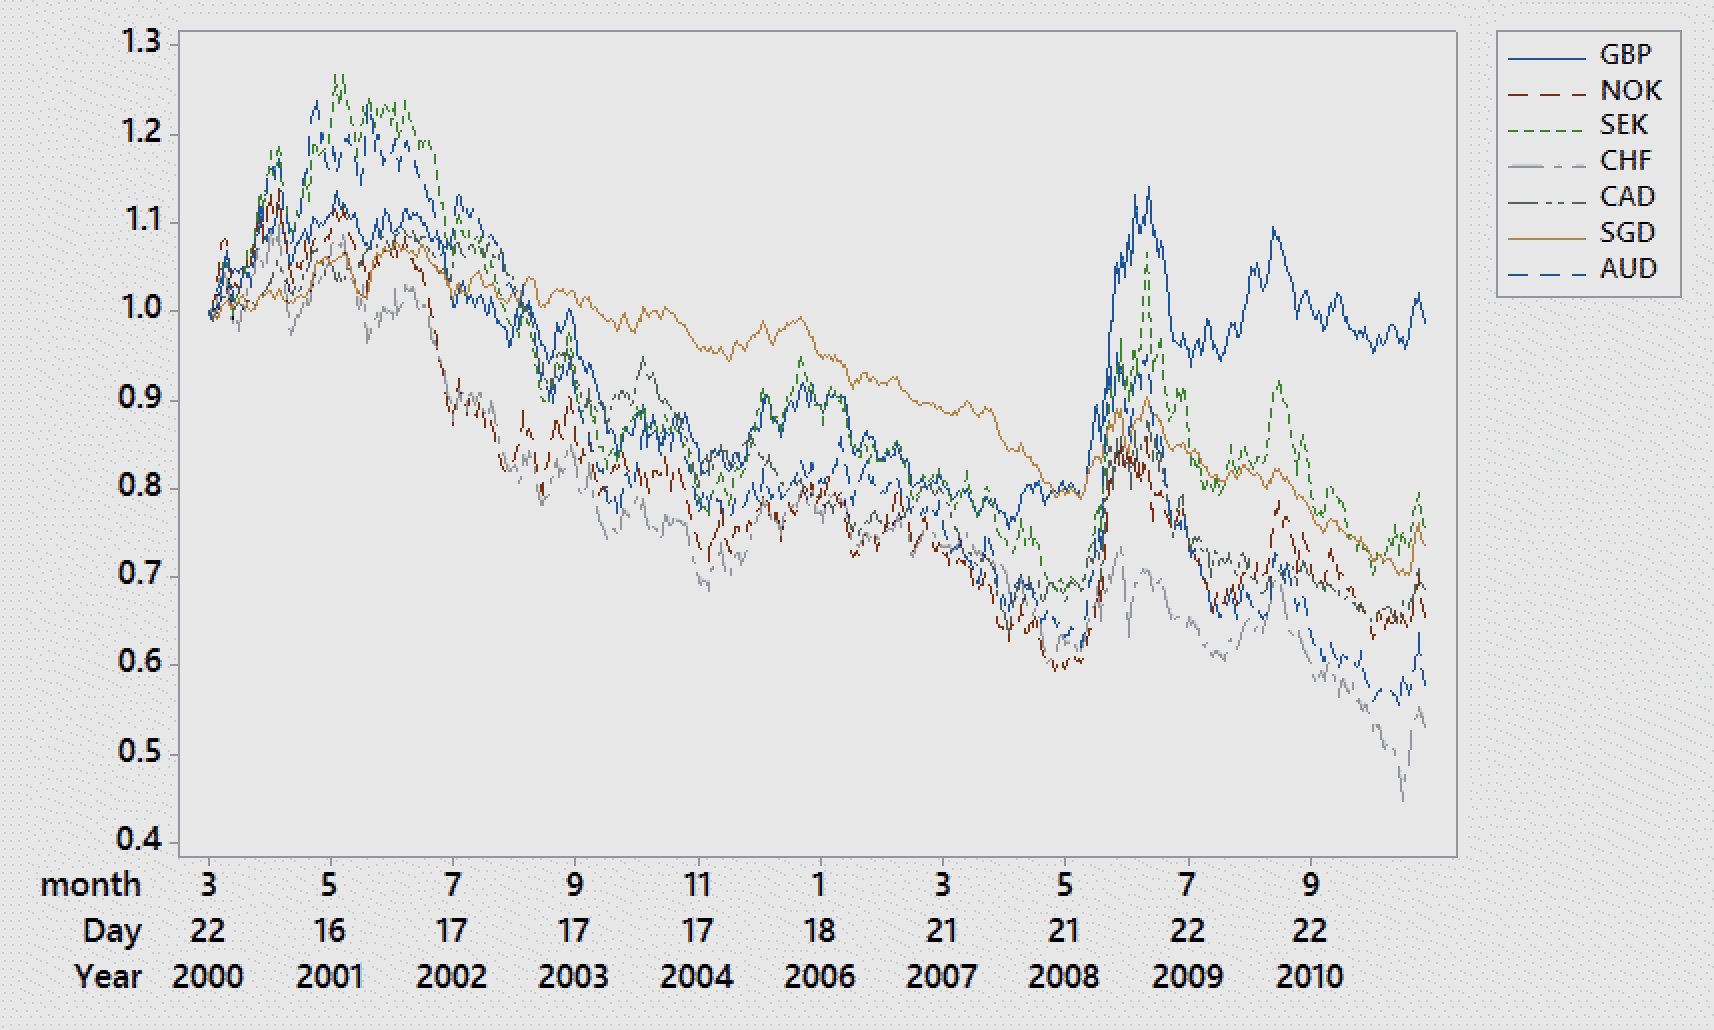
\includegraphics[width=\textwidth]{chapters/chapter_mvts/figures/exchangerates.png}
	\caption{Plot of Exchange Rates. \label{fig:exchrt}}
	\end{figure}


We consider the exchange rates of British Pound, Norwegian Kroner, Swedish Kroner, Swiss Franc, Canadian Dollar, Singapore Dollar, and Australian Dollar all stated against US Dollar. The weekly data is from March 22, 2000 to October 26, 2011 and it is the same data that was used in Hu and Tsay (2014)~\cite{hutsay14}. Thus $Y_t$ is a seven dimensional vector of time series. The return series $r_t$ is calculated as $r_t=\ln(y_t) - \ln(y_{t-1})$. The plot of $y_t$ is given in Figure~\ref{fig:exchrt} and to make the comparison easier, the first observation in all series are set to unity. Clearly the series are non-stationary and exhibit common upward and downward movements. The plot of returns and volatilities are given in Figures~\ref{fig:} and \ref{fig:}, respectively. They clearly indicate the periods of high volatilities in 2008--2009. 


\section{Exercises}













	
	

